\documentclass[a4paper]{article}
\usepackage{amsmath}
\usepackage{amsthm}
\usepackage[left=1.8cm,right=1.8cm,top=2.2cm,bottom=2.0cm]{geometry}
\usepackage{enumerate}
\usepackage{fancyhdr}
\usepackage{xpatch}
\usepackage{graphicx}
\usepackage{float}
\usepackage{subfigure}
\usepackage{amsfonts}
\usepackage{mathtools}
\usepackage{framed}
\usepackage{multicol}
\usepackage{fontspec}
\usepackage{float}
\usepackage{tikz}
\makeatletter

\printanswers


\AtBeginDocument{\xpatchcmd{\@thm}{\thm@headpunct{.}}{\thm@headpunct{}}{}{}}
\makeatother

\pagestyle{fancy}
\renewcommand{\baselinestretch}{1.15}
\newcommand{\code}[1]{\texttt{#1}}
\usepackage{paralist}
\let\itemize\compactitem
\let\enditemize\endcompactitem
\let\enumerate\compactenum
\let\endenumerate\endcompactenum
\let\description\compactdesc
\let\enddescription\endcompactdesc

% shorten footnote rule
\xpatchcmd\footnoterule
  {.4\columnwidth}
  {1in}
  {}{\fail}

\title{CSE 201: Homework 1}
% \author{\textbf{Yiwei Yang} \\ \texttt{ yyang363@ucsc.edu}}


\begin{document}
\maketitle
\section{Prove the $f(n)\in O(g(n))\cap \Omega(g(n))$ iff $\exists c_1>0,\exists c_2>0,\exists n_0>0, \forall n_0$ s.t. $0\leq c_1 g(n)\leq f(n)\leq c_2g(n)$}     
\begin{proof}
        \begin{enumurate}
                \item Suppose we have $f(n)\in O(g(n))\cap \Omega(g(n))$, from $f(n)\in O(g(n))$ we get $\exists c_1>0, \forall n_0 c_1g(n)\leq f(n)$, from $f(n)\in \Omega(g(n))$ we get $\exists c_2>0, \forall n_0 f(n)\leq c_2g(n)$. We proof that $\exists c_1>0,\exists c_2>0,\exists n_0>0, \forall n_0$ s.t. $0\leq c_1 g(n)\leq f(n)\leq c_2g(n)$
                \item Suppose we have $\exists n_1, c_1, \forall n \geq n_1, c_1 g(n) \leq f(n) $ and $\exists n_2, c_2, \forall n \geq n_2, f(n) \leq c_2 g(n)$. Let $n_0 = max(n_1, n_2)$, then we have $\forall n\geq n_0, 0\leq c_1 g(n)\leq f(n)\leq c_2g(n) $ ,$f(n)\in O(g(n))\cap \Omega(g(n))$
        \end{enumurate}
\end{proof}
\section{Find relation of following functions}
\subsection{$f(n)=2^n\quad  g(n)={(n lg(n))^2}$}
$f(n)=\omega(g(n))$
\begin{proof}
        $\frac{d}{d n}\left(\frac{2^n}{(n \lg (n))^2}\right) =\frac{2^n((n lg (2)-2) lg (n)-2)}{n^3 lg ^3(n)}$, Since $\frac {2^n}{n^3 lg ^3(n)}$ is monotonically increasing and bigger than 0 $\forall n > 0$, and $(n lg (2)-2) lg (n)-2$ is monotonically increasing and bigger than 0 $\forall n > 10$, Thus $\lim _{n \rightarrow \infty} \frac{f(n)}{g(n)}=\infty$, and $f(n)=\omega(g(n))$
\end{proof}
\subsection{$f(n)=\sqrt{n} \quad g(n)= lg (n)$}
$f(n)=\omega(g(n))$
\begin{proof}
        To proof $\exists c>0, \forall n>n_0$ s.t. $lg(n)\leq c\sqrt{n}$

        $\frac{d}{d n} \frac{\lg n}{\sqrt{n}}=\frac{2-\lg n}{2 n^{\frac{3} {2}}}$ for $n\geq e^2$, $\frac{f(n)}{g(n)}$ is decreasing, thus $c$ can be $\frac{2}{e}$.
\end{proof}
\subsection{$f(n)=(\lg n)^{(\lg n)}  \quad  g(n)=n^3$}
$f(n)=\omega(g(n))$
\begin{proof}
        $\frac{d}{d n}\left(\frac{\lg ^{\lg (n)}(n)}{n^3}\right)=\frac{\lg ^{\lg (n)}(n)(\lg (\lg (n))-2)}{n^4}$ Since $\frac {(\lg n)^{\lg n}}{n^{4}}$ is monotonically increasing and bigger than 0 $\forall n > e^e^2, \lg (\lg (n))-2$ is bigger than zeo, Thus $\lim _{n \rightarrow \infty} \frac{f(n)}{g(n)}=\infty$, and $f(n)=\omega(g(n))$
\end{proof}

\subsection{$f(n)=3^ {2^ n } \quad  g(n)=2^ {3^ n} $}
$f(n)=o(g(n))$
\begin{proof}
$\frac{d}{d n}\left(\frac{3^{2^n}}{2^{3^n}}\right)=2^{-3^n} \times 3^{2^n}\left(2^n-3^n\right) \log (2) \log (3)$. Since $2^n-3^n$ will be negative for $n>2$ and monotonically decreasing, and $2^{-3^n} \times 3^{2^n}$ is always positive, thus $\lim _{n \rightarrow \infty} \frac{f(n)}{g(n)}=0$, and $f(n)=o(g(n))$
\end{proof}

\subsection{$f(n)=n !  \quad  g(n)=(n+1) !$}
$f(n)=\omega(g(n))$
\begin{proof}
  $\lim _{n \rightarrow \infty} (n+1) ! /n !=\lim _{n \rightarrow \infty} \frac1n=0$, and $f(n)=o(g(n))$
\end{proof}
\subsection{$ f(n)=\lg \left(n^ n\right)  \quad  g(n)=\lg (n !)$}
$f(n)=\Theta (g(n))$
\begin{proof}
  Apply stirling's approximation
$$
\begin{gathered}
\lg (n !)=\lg \left(\sqrt{(2 \pi n}\left(\frac{n}{e}\right)^n\left(1+\Theta\left(\frac{1}{n}\right)\right)\right) \\
=\frac{1}{2} \lg (2 \pi n)+n \lg (n)-n \lg (e)+\lg \left(\Theta\left(\frac{n+1}{n}\right)\right)
\end{gathered}
$$
We know that the above equation is dominated by the second part. Thus they are $\Theta$ related.
\end{proof}
\section{Prove or disprove each of the following statements.} 
\subsection{Assume that $\lim _{n \rightarrow \infty} f(n)=\infty, \lim _{n \rightarrow \infty} g(n)=\infty, \forall n, f(n) \geq 1$ and $\forall n, g(n) \geq 1$. If $f(n)=O(g(n))$, then $\lg (f(n))=O(\lg (g(n)))$}\label{prove}
Approve
\begin{proof}
The condition $ f(n)=O(g(n))$, we have $\exists c>0, \forall n>n_0$ s.t. $f(n)\geq cg(n)$.

The condition $\lim _{n \rightarrow \infty} f(n)=\infty, \lim _{n \rightarrow \infty} g(n)=\infty$ makes c a bounded number got from 2 function are in the same order. 

\begin{figure}[h]
  \centering
  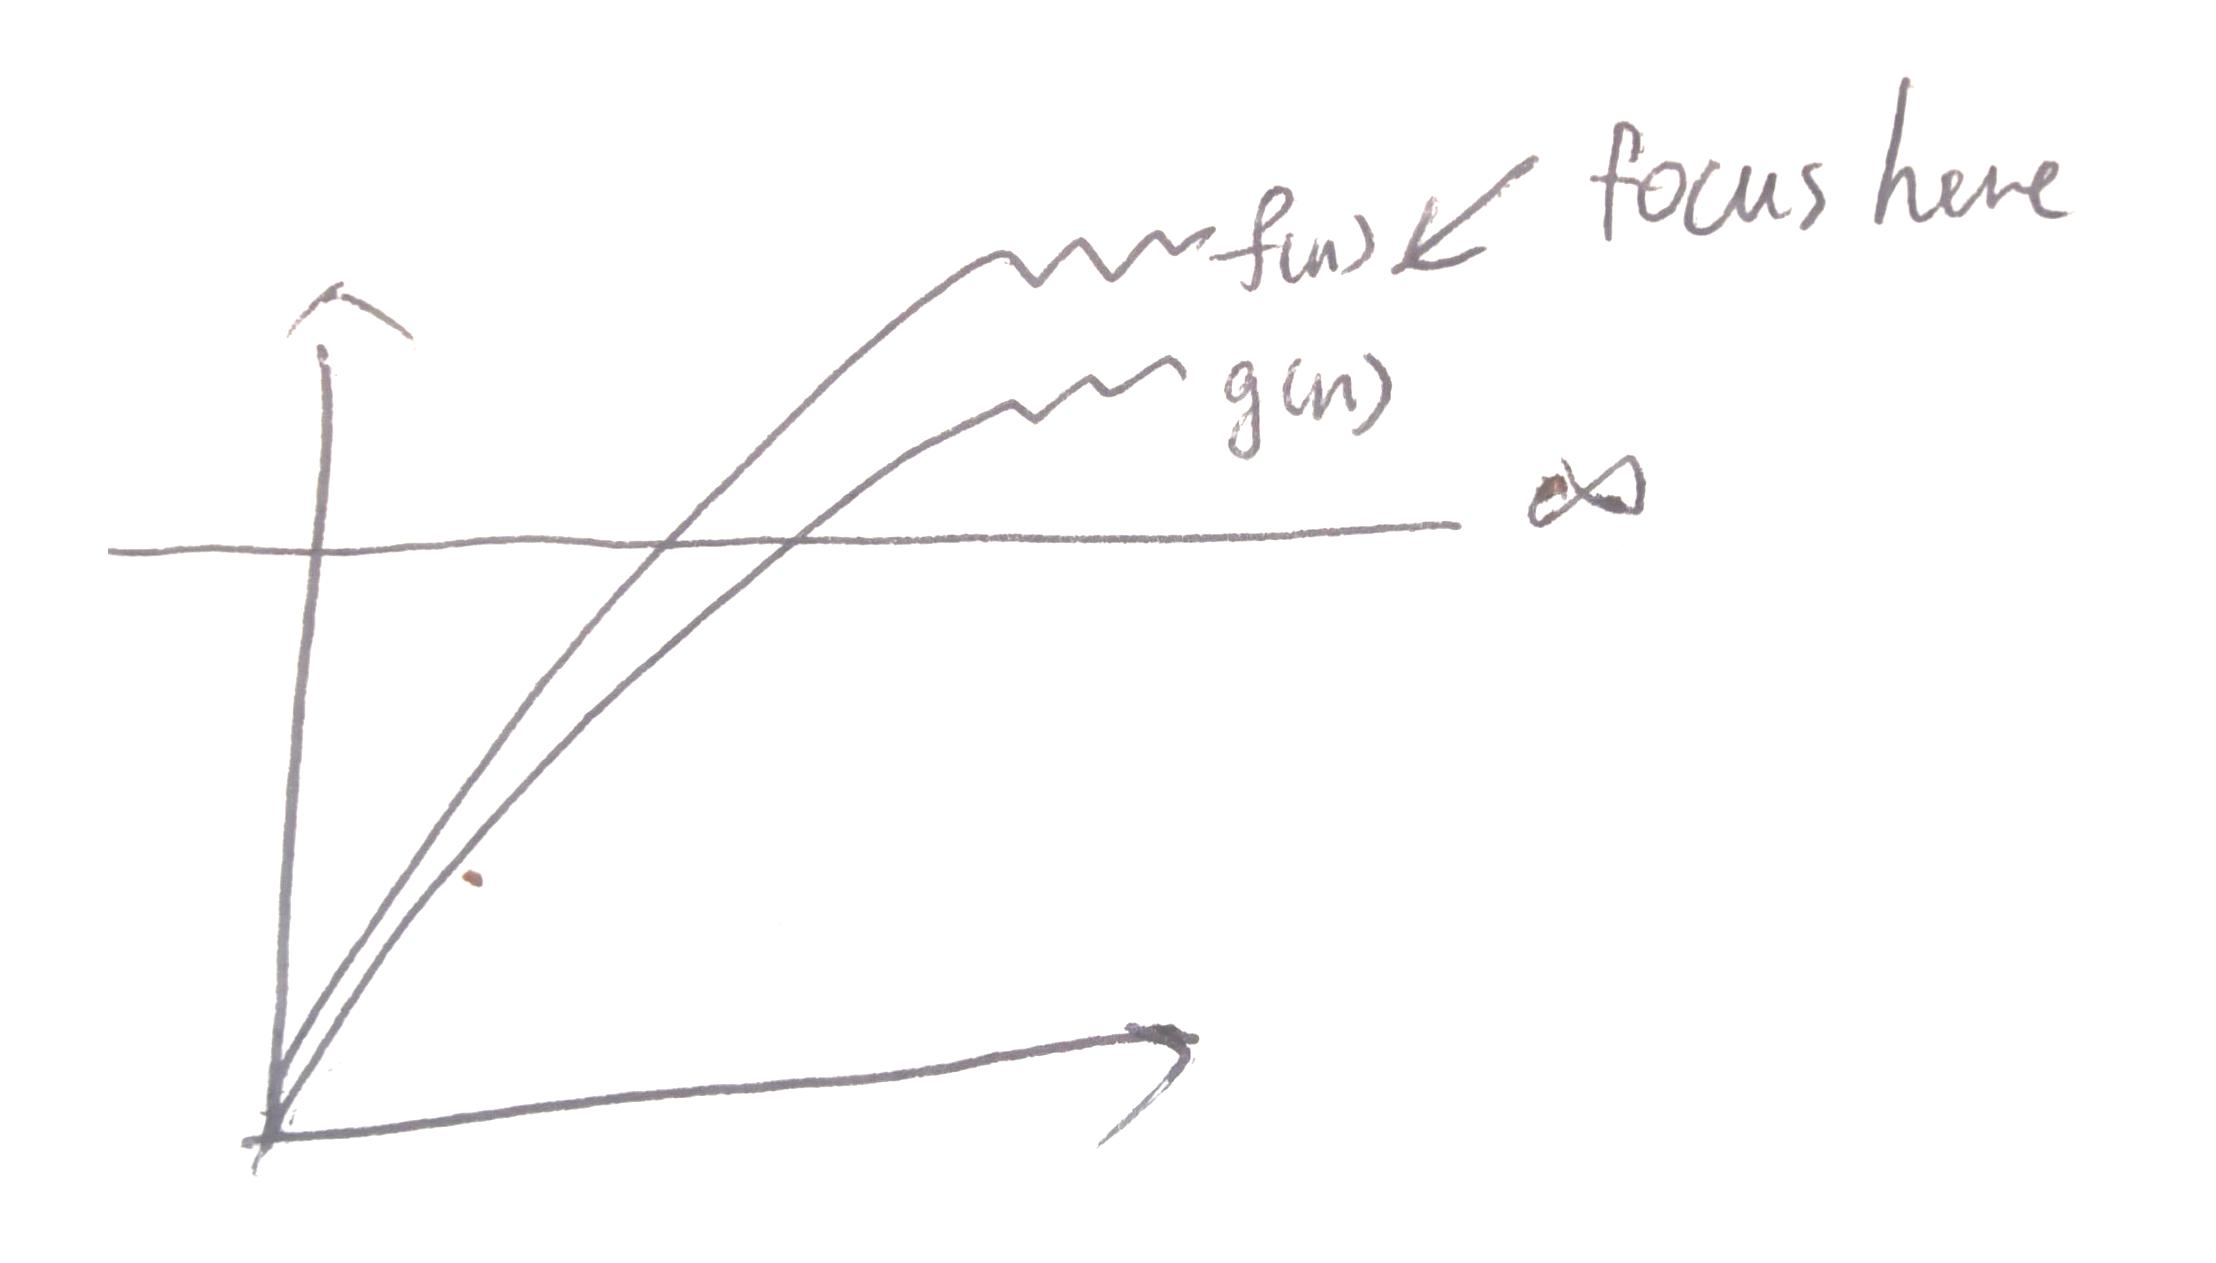
\includegraphics[width=0.4\linewidth]{./hw01-03-01.jpg}
\end{figure}

Suppose n is large enough s.t. $f(n)\geq 1$, $lg(f(n)) \leq lg(c g(n)) = lg(c) + lg(g(n))$
Let $c^{\prime}=lg(c)$: $lg(f(n)) \leq lg(g(n)) +c^{\prime}$

Suppose that $lg(g(n)) \geq \mu$ at large enough.
Then $(\frac{c^{\prime}}{\mu}+1)lg(g(n) \geq lg(g(n)) + c^{\prime}$
Thus $lg(f(n)) \leq c^{\prime\prime} lg(g(n)),$ where $c^{\prime\prime} = \frac{c^{\prime}}{\mu}+1$ 

Thus we found a $c$ that can make $\lg (f(n))=O(\lg (g(n)))$ happen.
\end{proof}
\subsection{ If $ f(n)=O(g(n)) $, then $2^{ f(n)}=O\left(2^ {g(n)}\right)$}
Disapprove
\begin{proof}
Suppose $f(n)=1.1n$, $g(n)=n$, we cant make $2^{1.1n}= 2^n$.
\end{proof}

\section{If $P(n)$ and $Q(n)$ are polynomials, with $degree(P) \leq degree (Q)$, and the leading coefficients of $Q(n)$ is positive, then $P(n) = O(Q(n))$.}
\begin{proof}
  Let $Q(n)= \Sigma_{0 \leq k\leq \text{degree}(Q)} a_k n^k, a_{\text{degree(Q)}>0}$, Let $P(n)= \Sigma_{0 \leq k\leq \text{degree}(P)} b_k n^k$, we have $\frac{d}{n} \frac{P(n)} {Q(n)}=a_{\text{degree}(Q)}\cdot{\text{degree}(Q)}\cdot n^{\text{degree}(Q)-1}+\text{remaining}>0,$ for $n\geq n_0$, thus $\lim _{n \rightarrow \infty} \frac{f(n)}{g(n)}=\infty$, thus $P(n)=O(Q(n))$.
\end{proof}
\section{Determine the asymptotic order of the expression $\sum_{i=1}^n a^i$ where $\mathrm{a} \in \mathbb{R}^{+}$. That is, find a simple function $\mathrm{g}(\mathrm{n})$ such that the above summation is in the class $\theta(g(n))$.}

\begin{proof}
  \begin{enumerate}
    \item $a\in (0,1)$, $\sum_{i=1}^n a^i = a^n+a^{n-1}\cdots +a=\frac{1-a^n}{1-a} a$, since, $\lim _{n \rightarrow \infty}\frac{1-a^n}{1-a} a=\frac{1}{1-a}a$, $g(n)=\frac{1}{1-a}a$
    \item $a=1$, $\sum_{i=1}^n a^i = 1+1\cdots+1=n$ $g(n)=n$
    \item $a\in (1,\infty)$, $\sum_{i=1}^n a^i = a^n+a^{n-1}\cdots +a= \frac{1-a^n}{1-a} a$, where the prime order for the function is contributed by $a^n$. $g(n)=\frac{a}{a-1}a^{n}$
    
  \end{enumerate}
  \end{proof}
\end{document}
